\documentclass[a4paper]{article}
\usepackage {changepage}
\usepackage{fancyhdr}
\usepackage {fontspec}
\usepackage {paralist}
\usepackage {multicap}
\pagestyle{fancy}
\setromanfont{Lantinghei SC Extralight}
\setmonofont{Courier New}
\XeTeXlinebreaklocale ``zh''
\XeTeXlinebreakskip = 0pt plus 1pt
\textheight = 650pt
\begin{document}
\title{TCP Introduction}
\author{姓名:王钦\quad 学号:13349112}
\date{}
\maketitle

\section*{ 概述}
\hangindent=3em \hangafter=-100{
\indent TCP 是传输控制协议一种面向连接的、可靠的、基于字节流的传输层通信协议,由IETF的RFC 793定义。在简化的计算机网络OSI模型中,它完成第四层传输层所指定的功能,用户数据报协议(UDP)是同一层内,另一个重要的传输协议。在因特网协议族中,TCP层是位于IP层之上,应用层之下的中间层。不同主机的应用层之间经常需要可靠的、像管道一样的连接,但是IP层不提供这样的流机制,而是提供不可靠的包交换。
}
\section*{ 连接建立(三次握手)}
\hangindent=4em \hangafter=-200{
	  \begin{itemize}
		  \item 客户端发送SYN(SEQ=x)报文给服务器端,进入SYN\_SEND状态。
			\begin{center} 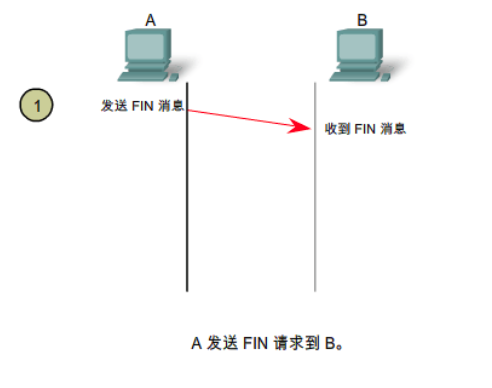
\includegraphics[scale=0.3]{Illustrations/tcp01.png} \end{center}
		  \item 服务器端收到SYN报文,回应一个SYN (SEQ=y)ACK(ACK=x+1)报文,进入SYN\_RECV状态。
			\begin{center} 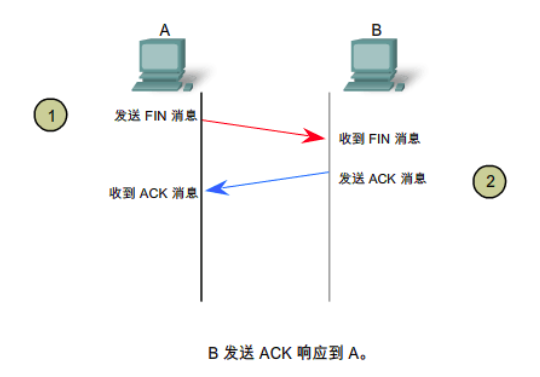
\includegraphics[scale=0.3]{Illustrations/tcp02.png} \end{center}
		  \item 客户端收到服务器端的SYN报文,回应一个ACK(ACK=y+1)报文,进入Established状态。
			\begin{center} 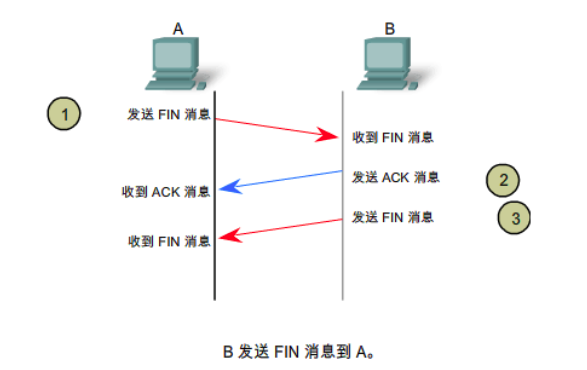
\includegraphics[scale=0.3]{Illustrations/tcp03.png} \end{center}
		  \item 三次握手完成,TCP客户端和服务器端成功地建立连接,可以开始传输数据了。
			\begin{center} 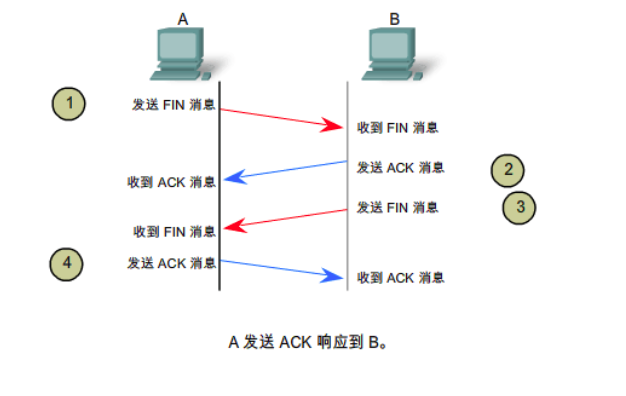
\includegraphics[scale=0.3]{Illustrations/tcp04.png} \end{center}
	  \end{itemize}
}

\section*{ 连接终止(四次握手)}
\hangindent=4em \hangafter=-200{
	  \begin{itemize}
		  \item 某个应用进程首先调用close,称该端执行“主动关闭”(active close)。该端的TCP于是发送一个FIN分节,表示数据发送完毕。
		  \item 接收到这个FIN的对端执行 “被动关闭”(passive close),这个FIN由TCP确认.
		  \item 一段时间后,接收到这个文件结束符的应用进程将调用close关闭它的套接字。这导致它的TCP也发送一个FIN。
		  \item 接收这个最终FIN的原发送端TCP(即执行主动关闭的那一端)确认这个FIN.
		  \item 四次握手完成,TCP客户端和服务器端终止连接.
		\begin{center} 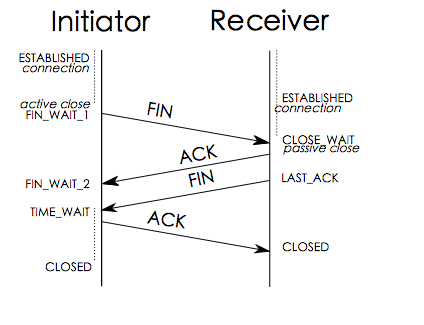
\includegraphics[scale=0.5]{Illustrations/tcp1.png} \end{center}
	  \end{itemize}
}
\section*{ TCP头格式}
\hangindent=4em \hangafter=-200{
	  \begin{itemize}
		  \item TCP的包是没有IP地址的,那是IP层上的事。但是有源端口和目标端口。
		\begin{center} 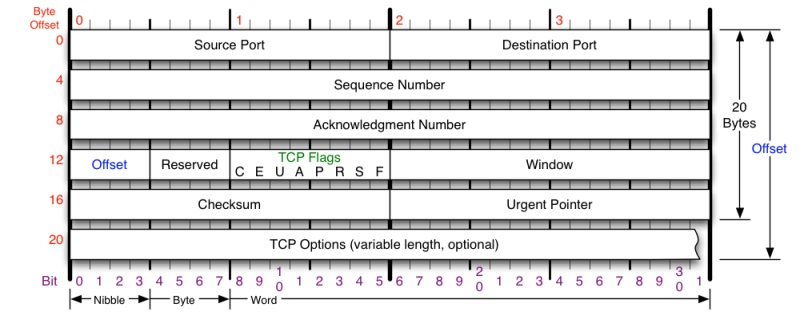
\includegraphics[scale=0.5]{Illustrations/tcp_head.jpg} \end{center}
		  \item 一个TCP连接需要四个元组来表示是同一个连接(src\_ip, src\_port, dst\_ip, dst\_port)准确说是五元组,还有一个是协议。但因为这里只是说TCP协议,所以,这里我只说四元组。
		  \item Sequence Number是包的序号,用来解决网络包乱序(reordering)问题。
		  \item Acknowledgement Number就是ACK——用于确认收到,用来解决不丢包的问题。
		  \item Window又叫Advertised-Window,也就是著名的滑动窗口(Sliding Window),用于解决流控的。
		  \item TCP Flag ,也就是包的类型,主要是用于操控TCP的状态机的。
	  \end{itemize}
}
\section*{ TCP重传机制}
\hangindent=4em \hangafter=-200{
	  \begin{itemize}
		\item TCP要保证所有的数据包都可以到达,所以,必需要有重传机制。注意,接收端给发送端的Ack确认只会确认最后一个连续的包,比如,发送端发了1,2,3,4,5一共五份数据,接收端收到了1,2,于是回ack 3,然后收到了4(注意此时3没收到),此时的TCP会怎么办?我们要知道,因为正如前面所说的,SeqNum和Ack是以字节数为单位,所以ack的时候,不能跳着确认,只能确认最大的连续收到的包,不然,发送端就以为之前的都收到了。
		\item 超时重传机制,一种是不回ack,死等3,当发送方发现收不到3的ack超时后,会重传3。一旦接收方收到3后,会ack 回 4——意味着3和4都收到了。
		    但是,这种方式会有比较严重的问题,那就是因为要死等3,所以会导致4和5即便已经收到了,而发送方也完全不知道发生了什么事,因为没有收到Ack,所以,发送方可能会悲观地认为也丢了,所以有可能也会导致4和5的重传。
		\item 快速重传机制TCP引入了一种叫Fast Retransmit 的算法,不以时间驱动,而以数据驱动重传。也就是说,如果,包没有连续到达,就ack最后那个可能被丢了的包,如果发送方连续收到3次相同的ack,就重传。Fast Retransmit的好处是不用等timeout了再重传。
		    比如:如果发送方发出了1,2,3,4,5份数据,第一份先到送了,于是就ack回2,结果2因为某些原因没收到,3到达了,于是还是ack回2,后面的4和5都到了,但是还是ack回2,因为2还是没有收到,于是发送端收到了三个ack=2的确认,知道了2还没有到,于是就马上重转2。然后,接收端收到了2,此时因为3,4,5都收到了,于是ack回6。示意图如下:

		\begin{center} 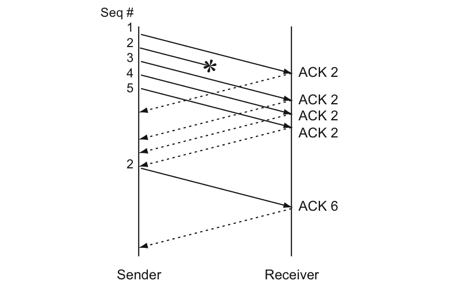
\includegraphics[scale=1]{Illustrations/retransmit.png} \end{center}
		\item SACK 方法,另外一种更好的方式叫:Selective Acknowledgment (SACK)(参看RFC 2018),这种方式需要在TCP头里加一个SACK的东西,ACK还是Fast Retransmit的ACK,SACK则是汇报收到的数据碎版。参看下图:
		\begin{center} 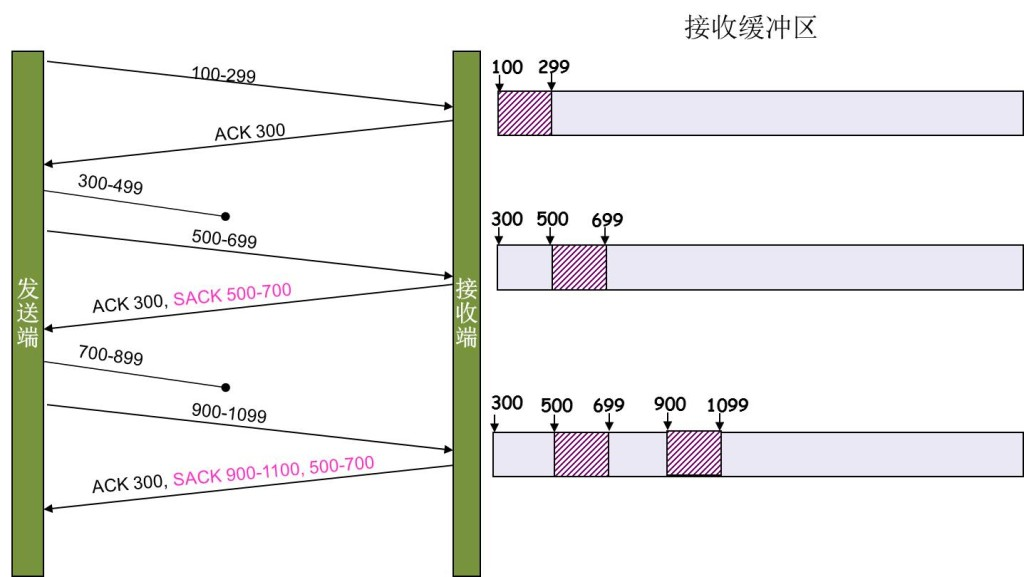
\includegraphics[scale=0.5]{Illustrations/sack.jpg} \end{center}
	  \end{itemize}
}
\section*{ TCP和UDP区别}
\hangindent=4em \hangafter=-200{
	  \begin{itemize}
		\item 基于连接与无连接;
		\item 对系统资源的要求(TCP较多,UDP少);
		\item UDP程序结构较简单;
		\item 流模式与数据报模式 ;
		\item TCP保证数据正确性,UDP可能丢包,TCP保证数据顺序,UDP不保证。
	  \end{itemize}
}

\end{document}



